\chapter{Action--sound mappings}\label{chapter:mappings}

`We hear new sounds, we see familiar sounds coming out of unfamiliar devices, and unfamiliar sounds coming out of familiar interfaces.` writes \citet{kvifte_what_2008} in a discussion of the changing nature of musical instruments. Indeed, today's new instruments are in many ways different from the traditional instruments we are accustomed to performing and perceiving. Yet, as the discussion in the last chapter showed, traditional instruments also differ. New acoustic instruments are still invented, but there are many more new electro-acoustic instruments. The latter is based on designing and constructing action--sound \emph{mappings}. In electro-acoustic instruments, the interaction is created by transferring electric signals (analog or digital) in a chain of interconnected devices, such as sketched in Figure~\ref{fig:electroacoustic2}. I will argue that there are both practical and conceptual differences between instruments based on couplings and mappings. Not least do electro-acoustic instruments allow for even more explorations into both sound-making and music-making.

\begin{figure}[tp]
	\centerline{
		  
\includegraphics[width=.9\textwidth]{figures/46-mapping-crop.pdf}
			\caption{An electro-acoustic instrument can be broken into three core components: controller, sound engine, and speaker.}
			\label{fig:electroacoustic2}
}
\end{figure}


\section{From electro to acoustic}

Before moving on, it may be worth repeating my rationale for using the term electro-acoustic instrument. The \emph{electro} part of the term refers to the need for electric power to produce sound in such instruments. The \emph{acoustic} part refers to the fact that these instruments produce audible sound. I stress this because I find that the final sounding sound is often neglected in the literature on instruments. Even the legendary synthesizer builder Bob Moog `forgot' about the sound-producing element when he summarized the three determinants of musical instrument design \citep{roehmann_biology_1988}:

\begin{quote}
	The first is the sound generator; the second is the interface between the musician and the sound generator; the third is the [\ldots] visual reality of the instrument.
\end{quote}

I agree with Moog that the sound generator---what I will call a \emph{sound engine}---is a central part of an electro-acoustic instrument. As sketched in Figure~\ref{fig:electroacoustic2}, the sound engine is controlled by a performer's actions. These actions are picked up by sensors in a physical \emph{controller}. Finally, the sound is produced by a \emph{speaker} element, typically connected to an amplifier.

What differentiates electro-acoustic instruments from acoustic is the lack of a direct, physical energy transfer from the performer to the final sound. The performer uses energy on the controller, but this is not the same energy used to produce sound coming out of the speaker. Instead, the instrument relies on energy from an external power source. This is not a problem per se, but it is a different concept---and technological construction---than what is found in an acoustic instrument.
In electro-acoustic instruments, the parts in the chain are usually functionally independent. This allows for customization since controllers, sound engines, and speakers can be chained differently. While this is one of the strengths of electro-acoustic instruments, it is also one of their conceptual drawbacks.

\citet[4]{miranda_new_2006} argue that \emph{mappings} between the performer's action and the sound generating device are central to \emph{digital} electro-acoustic instrument design. I would argue that mapping is also vital for \emph{analog} electro-acoustic instruments, although there are some differences between analog and digital circuitry. However, these differences are much more minor than the differences between electro-acoustic and acoustic instruments. Action--sound mappings are \emph{designed}. One may say that the couplings found in acoustic instruments are also `designed' in that various sound-producing objects are put together in a particular way. In acoustic instruments, however, the resultant sound is based on the inherent physical properties of its sound-producing objects. In electro-acoustic instruments, the mappings created between a controller and a sound engine are arbitrary and may confuse both performers and perceivers. As the last decades of research into new interfaces for musical expression have shown, many instrument builders strive to create meaningful mappings in their electro-acoustic instruments.

\section{The parts of an action--sound chain}

Before moving on to some concrete examples, we will look more closely at each of the parts of the mapping chain described above. These are summarized in Figure~\ref{fig:electroacoustic3}. We will consider the sound-producing parts first and then move on to the controller and mappings between action and sound.

\begin{figure}[tbp]
	\centerline{
		  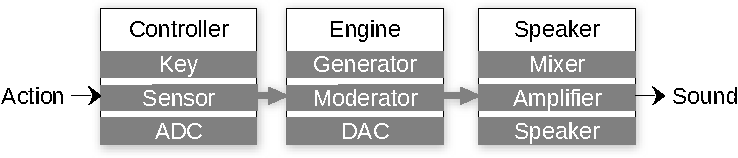
\includegraphics[width=\textwidth]{figures/47-mapping2-crop.pdf}
			\caption{A schematic overview of some parts making up a controller, sound engine, and speaker.}
			\label{fig:electroacoustic3}
}
\end{figure}


\subsection{The sound engine}

The sound engine is at the core of any electro-acoustic instrument. After all, this is where sound generation occurs. Broadly speaking, we can talk about \emph{analog} and \emph{digital} electro-acoustic instruments. That is, instruments that produce sound through either analog circuitry or digital code. I have chosen this terminology to avoid the terms `electric' and `electronic' instruments. Any instrument powered from electricity could be called electric. An electronic system, on the other hand, is based on manipulating electrical current through switches. This is how most analog electro-acoustic instruments are constructed. Many of these are built around one or more \emph{oscillators}, an electronic circuit that produces a periodic, oscillating electronic signal. An oscillator converts direct current from a power supply to an alternating current signal, resulting in a sine tone or square wave. There are only a few instruments that would be categorized as purely electric. One of these is the Victorian Synthesizer \citep{collins_handmade_2009}, which we will get back to soon. Most analog electro-acoustic instruments, however, could be classified as electronic.

When it comes to \emph{digital} systems, it is worth mentioning that technically speaking, such a system would be a sub-category of both electric and electronic. Digital systems are electric since they run on electricity, and they are electronic because they are based on electronic circuitry. The difference is that the electronic circuits used in digital instruments operate with binary logic (ones and zeros). An electro-acoustic instrument based on digital processing is built around a discretization of sound signals. This involves an analog-to-digital converter (ADC) for sound recording and a digital-to-analog converter (DAC) for sound production. It could be argued that the discretization process in digital instruments makes them inferior to the (in theory) continuous signal of analog instruments. However, today's ADC/DAC converters run at sample rates and with bit depths higher than the limits of the human auditory system. So there is no practical difference between analog and digital circuitry any longer. The main theoretical difference is that the signal is passed through the system in analog circuitry without any discretization. This has some practical implications. Digital sound-processing has revolutionized the industry, allowing for noiseless recording, mixing, copying, and transmission of musical sound. Interestingly, despite the many positive sides of digital sound processing, there is a continuous demand for analog devices. Some people argue that imperfections of analog circuitry make the sound `richer' \citep{jenkins_analog_2007}. Others complain about the delay---measured as the \emph{latency}---of digital systems \citep{jota_how_2013}.

Acoustic instruments can often be broken down into sound-producing and sound-modifying elements. The same is the case for electro-acoustic instruments. Many synthesizers are built around the concept of sound \emph{generators}, such as different types of waveforms (sine, square, noise, and so on). The sound coming out of the generator can be fed into a \emph{moderator}. For example, a filter can shape a sound's timbral qualities, while envelopes and low-frequency oscillators shape its temporal development. Many systems also play with feedback loops between generators and moderators. This allows for creating complex timbres, textures, or rhythmic patterns.


\subsection{The speaker}

In his foreword to the book \emph{Material culture and electronic sound} \citep{weium_material_2013}, Brian Eno eloquently describes his thoughts on the importance of speakers:

\begin{quote}
So modern electronic instruments are incomplete without their `bodies'---the amplifiers and loudspeakers by which they're heard. [\ldots] Before the amp and speakers; it's all about numbers.
\end{quote}

Eno writes `numbers' here, by which I take it that he refers to digital devices. However, also for non-number-based (analog) electro-acoustic instruments, there is no sound without a speaker. As sketched in Figure~\ref{fig:electroacoustic3}, a speaker also typically needs one or more amplifiers to produce audible sound. I have also added a mixer to the chain, since that is often needed to route signals correctly. The mixer may also act as a sound-modifying device on its own.

Generally speaking, we may separate speakers that produce sound waves in the air from those that make sound through a physical object's vibrotactile stimulation. The first is what is found in most loudspeakers, in which the loudspeaker cone moves and creates sound waves in the air. When people ask me why I am interested in music-related body motion, I ask them to touch a speaker element. Feeling the vibration of a speaker element is a way of `touching' the sound. It is also an efficient reminder that sound is vibration. Normal loudspeaker elements produce vibrations in the air. Vibrotactile speakers, on the other hand, produce vibrations in physical objects. Here the final sound is heavily influenced by the acoustic properties of the object in question. For example, adding vibrotactile speakers to an acoustic guitar body is different from trying to excite a concrete wall. Most electro-acoustic instruments are still based on loudspeakers producing sound in the air. However, there has been an increased interest in \emph{hybrid instruments} in recent years \citep{lahdeoja_augmented_2015,eldridge_self-resonating_2017,NIME20_42}. These are based on creating vibrations in acoustic objects based on analog and digital circuitry connected to vibrotactile speakers.

Headphones is a speaker category that receives little research attention despite their musical impact. Many people perceive music through headphones, and many musicians playing electro-acoustic instruments spend a great deal of time rehearsing with headphones. Many musicians also perform with headphones these days. Then I include all sorts of headphones: in-ear, over-ear, around-ear, and bone-conductive. The latter is a particular category, but the others have in common that they primarily transmit sound directly to the ear. This is different from other types of speakers, which also transmit sound waves to the body. Everyone that has stood in front of a large PA system can attest to the bodily sensation of the sound waves. Given their widespread usage, I am puzzled why there are so few studies on the differences between headphones and speakers. For that reason, we carried out an experiment at the University of Oslo in which participants stood still while listening to music through either headphones or speakers. Interestingly, we found that people systematically moved more when listening to headphones than speakers \citep{zelechowska_headphones_2020}. This, we believe, can be explained by the `closing off' of one sense. Just as one gets more unstable by closing the eyes, putting on headphones removes much contextual information about the space one is standing in. This again may affect the balance. In our experiment, we used loud but comfortable sound playback levels from both loudspeakers and headphones. So the energy of the sound waves presented through loudspeakers was not enough to physically move people. It would be interesting to know more about how much people are actually moved when listening to loud music in front of a large PA system.

Bone-conducting headphones are an exciting in-between speaker technology. This is not a new type of device, but we have seen more commercial interest in such products in recent years. Particularly for people that need to keep attention to their audible surroundings, such as joggers, this type of device is useful. Bone-conducting headphones are not placed over the ears but rather on the chin. The vibrotactile stimulation makes it possible to hear sound and music quite satisfactory, although not with the same fidelity level as one would expect from a regular pair of headphones. I find it both strange and fascinating to wear such headphones. You have an intimate sound experience while also hearing everything else in the environment. Such headphones allow for perceiving the `outer' world while at the same time having an `inner' experience of music. While headphones are attractive in many ways and deserve more research attention in general, I will primarily focus on loudspeakers in the rest of this book.

Looking at the sketch of equipment in Figure~\ref{fig:electroacoustic3}, the chain may be short if the sound engine is connected directly to the speaker. However, the sound may be passed from the sound engine to a mixer, connected to an amplifier and the speaker. In active speakers, the amplifier is built into the speaker cabinet, but it is still there. There may be multiple layers of mixers, DI boxes, and amplifiers going into a large speaker rig in larger concert setups. This usually also impacts the sound in one or more ways. If the chain is based on passing analog signals, this may `color' or distort the sound. Using digital mixers help in avoiding such artifacts but may introduce latency. Also, like for acoustic instruments, it is essential to consider the space within which an instrument is played. Electro-acoustic instruments are also played in spaces with acoustic features. In addition, it is common to add virtual space information to the mix. We will look more at how such equipment chains may increase (or decrease) the perceived spatiotemporal distance in Chapter~\ref{chap:hybrid}.


\subsection{The controller}

The controller is the device that captures the performer's action and passes it on to the sound engine. At the core of a controller is a \emph{sensor} that converts physical energy into an electric signal, what \citet{bongers_physical_2000} calls the `sense organ' of the system.
In some cases, the user may be in contact with the sensor directly. More often, the sensor is covered by some mechanical moving parts, such as the keys on a keyboard-based controller. As reviewed by \citet{medeiros_comprehensive_2014}, numerous sensor types are used for musical applications. They can be \emph{discrete}, such as, on/off-type capacitance sensors, or \emph{continuous}, such as, force-sensing resistors (FSRs). Light sensors and temperature sensors can be used, although they are often too slow for musical interaction. Then various infrared sensors may be more practical, either used as on/off-switches or for continuous control. As described in Chapter~\ref{sec:motion-capture}, various types of motion tracking systems are also increasingly used in interactive music systems.

No matter what type of sensor is used, it needs to be connected to the rest of the circuitry through a \emph{sensor interface}. A sensor interface typically contains an analog-to-digital converter (ADC) that converts the electric sensor signal to a binary control signal in a digital instrument. For most physical controllers, for example, keyboards, there would usually be many mechanical parts, each connected to one or more sensors. There may also be multiple sensor interfaces on the inside, although the end-user may only see a single stream of controller values that can be mapped further.

There has always been much experimentation with different types of controllers for both analog and digital instruments. \citet{miranda_new_2006} suggest four categories: (1) augmented musical instruments, (2) instrument-like controllers, (3) instrument-inspired controllers, (4) alternate controllers. This is a good summary of controllers found in the music technology research community. However, looking at commercially available controllers, the vast majority of products fall into one of these categories (or a combination of these):

\begin{description}
	\item[keyboard-like controllers:] typically modeled after the piano, with its black and white keys.
	\item[mixer-like controllers:] built using the `knobs-and-sliders' paradigm found in most mixers.
	\item[pad-like controllers:] controllers built around a grid of touch-sensitive buttons.
  \item[acoustic-instrument-like controllers:] for example drum kits and wind controllers.
\end{description}

As described in Chapter~\ref{sect:midi}, the MIDI standard has been successful in allowing for setting up any type of connection between controllers and sound engines. But its focus on impulsive note-on/note-off messages may also be one of the reasons why most of the above-mentioned controller types (minus the few wind controllers out there) are built around sensors that work well within a MIDI-based control paradigm.

Fortunately, the music technology research community is actively developing new prototypes, with the annual International Conference on New Interfaces for Musical Expression (NIME) being the most central dissemination channel \citep{jensenius_nime_2017}. We will look more at some of my contributions to this community in Chapters~\ref{chap:unconventional} and \ref{chap:touchless}.


\subsection{Mappings}

As mentioned above, we may think of \emph{mappings} as the `glue' between the three main parts of electro-acoustic instruments: controllers, sound engines, and speakers. In its technical sense, mappings describe individual control parameters' connections to individual sound synthesis parameters. We may also think about mappings in a techno-cognitive sense: the experienced relationships between actions and sounds. This is the way I use the term when talking about action--sound mappings. The technical and conceptual levels are, of course, related. Ideally, a conceptual mapping idea is realized in the technical mapping.

\citet[p.171]{levitin_control_2002} start their discussion on strategies for developing new instruments with three postulates:

\begin{itemize}
 \item Suitable mappings must be found between a musician’s gesture and the control of various aspects of a musical tone \citep{cadoz_responsive_1984,wanderley_performer-instrument_2001}.
 \item Gestures are motions of the body that contain information \citep{kurtenbach_gestures_1990}.
 \item Mappings are best when they are intuitive, and when they afford the maximum degree of expression with minimal cognitive load \citep[e.g.][]{keele_attention_1973,mulder_mapping_1997}.
\end{itemize}

Although I use slightly different terminology, these postulates resonate well with my action--sound theory.
When it comes to creating mappings, this may happen at multiple stages throughout the design phase. At the most technical level, deciding which sensors to include in the controller may be seen as part of the mapping process. While any standard industrial sensor may be used for musical applications, \citet{kronland-martinet_evaluation_2006} have argued that it is essential to evaluate sensors with respect to their intended application. For example, a bend sensor may be used to control anything from pitch to loudness. Still, it may not be the best sensor considering the controller's actions or the parameters available in the sound model. An intuitive instrument design should be based on developing a controller that captures the intended actions. This should be followed by choosing a sound synthesis model with input parameters that fit the controller's outputs. The result would be action--sound mappings that work well for the performer and are intuitive for the perceivers.

On the sound engine side, there are many initial mapping decisions to be made. A typical sound synthesis model consists of many technical parameters. These do not necessarily correlate directly to perceptual qualities. A standard solution to master such a complex system is to create presets that define a set of parameters that work well together. These presets may then be used for further exploration of the sound synthesis model. However, the drawback of such a design decision is that users may end up using only presets. This may or may not be a problem, but it should be considered during the design phase.

While many commercial electro-acoustic instruments are heavily preset-based, there has been much exploration with different mapping strategies in the music technology research community.
When I teach electro-acoustic instrument design, students often start by creating one-to-one mappings between the controller and the sound engine. Connecting a slider to a sine tone generator is one of the most classic examples. Such a basic mapping makes sense from a technical perspective. One could even argue that the sensor and sound engine afford such a one-to-one mapping. For the user, it may make sense to have direct control of the sound, although it seldom leads to impressive musical results. \citet{kvifte_instruments_1989} has argued that many acoustic instruments are, in fact, based on \emph{coupled} mappings. For example, the breath of a clarinetist may control the timbre, loudness, and vibrato of the sound simultaneously. Similarly, these sound parameters may also be controlled by lip pressure. Many acoustic instruments are based on one-to-many or many-to-one mappings. In studies of people's experiences of different types of mappings, \citet{hunt_mapping_2002} found that people often find such coupled mappings to be more intuitive and exciting than more straightforward one-to-one mappings. The study confirmed that what might seem to be an efficient mapping strategy from an engineering point of view may not be the best from a musical perspective.

There are also numerous examples of more complex many-to-many mapping solutions. For example, \citet{momeni_characterizing_2003} suggested using a three-dimensional geometrical representation to control a highly multidimensional sound synthesis engine by interpolating values coming from a graphic tablet. \citet{dahlstedt_mutasynth_2001} developed a system in which an evolutionary algorithm would generate new presets by keeping some information from the previous presets. In this way, it was possible to generate a set of presets with similar characteristics to the presets of the `parents.' Another approach to controlling complex sound models was suggested by \citet{bevilacqua_gesture_2005}, who used statistical models to learn mappings between multidimensional control parameters and sound synthesis parameters. In that system, the user would make an action with a controller and select some sound synthesis parameters that the action should control. The model would also interpolate between different actions, which would result in combinations of the assigned sound synthesis parameters.

Although artificial intelligence (AI) methods have been around for decades, it is only more recently that it has been possible to work with machine learning in musical applications \citep{inesta_machine_2018}. Such models can be trained before a performance, but tools like Wekinator make it possible to use machine learning in real-time \citep{fiebrink_wekinator_2010}. This allows for creating complex many-to-many mappings during performances. The development of musical deep learning methods will probably further drive the mapping possibilities in future instruments \citep{briot_deep_2019}.
A compelling aspect of such AI-based systems is that they do not require knowledge about the mapping parameters. The mappings are created automatically based on examples given by the user. That may work well, but it also provides the user with less direct control of the instrument.

The above-mentioned approaches are often based on `point-wise' mappings, defining points (presets) in a multidimensional space relating control and sound synthesis parameters. \citet{van_nort_modular_2010} argued that one should not only define \emph{what} to map but also \emph{how} it is mapped. The trajectories between points in a mapping space may change the `feel' of a controller. Anyone who has switched between logarithmic and linear mapping knows how different they feel in practice. So one could argue that a controller's perceived expressivity is linked to the dynamic quality of its mappings.

\emph{Physical modeling} is a conceptually different approach to mapping than the examples mentioned above. Creating models that reflect the underlying physical sound production may be seen as an `ecological' approach to sound synthesis. In such models, the control parameters are inspired by physical actions and objects rather than some abstract technical parameters.
Physical modeling synthesis was first proposed by \citet{karplus_digital_1983}, and their original model is commonly referred to as Karplus-Strong string synthesis. This physical model aims to simulate the pluck of a string by sending a burst of white noise into a filtered delay line. The result is a remarkably rich sound, particularly given the few elements of the algorithm. What is fascinating about physical modeling, as opposed to techniques such as additive synthesis, is that the user can `excite' the model by sending noise bursts into the delay line. This can be seen as analogous to performing multiple `plucks' on a physical string. Since the Karplus-Strong model is based on a delay line, one may continue to re-excite the model before the sound has decayed. This will build up the resonance in the model, just as you would experience with an actual resonating string. As such, a physical sound model behaves quite similarly to real-world sound excitation. This is quite different from, for example, sample-based sound engines, in which one always talks about the `polyphony' of the system as the main limitation for the sonic richness that it is possible to achieve.

Since a physical model is developed based on the imagined physical properties of the actions and objects involved, it calls for a direct mapping process in which the controller's physical outputs may be mapped directly to the input parameters of the sound model. An early example of a physical modeling approach to musical instrument design is the CORDIS system by \citet{cadoz_responsive_1984}. While physical modeling has yet to reach its full commercial potential, research progress have been made with the development of \emph{digital waveguide synthesis} by \citet{smith_physical_1992} and \emph{physically inspired stochastic event modeling} (PHISM) and related controllers developed by \citet{cook_principles_2001}. There are also examples of how physical modelling can be used creatively to set up unintuitive mappings. \citet{li_study_2020} explored using a single-reed woodwind controller with a bowed string synthesis engine. This is an odd combination, but less so than using an impulsive controller with a sustained sound model. At least, the setup allowed for continuous control of the sound engine.

Much more could be said about mappings; in fact, \citet{baalman_just_2021} currently writes a book on the topic. My main point is to stress that mappings are integral to the design of an electro-acoustic instrument. It is also a central part of the creative process when working with electronics in a musical context. While mapping has received more interest in the research domain in recent years, there is still much work that needs to be done both theoretically and practically. There is much creative potential in the development of new and better mappings between action and sound. There are also numerous scientific insights to be gained through studies of mappings. After all, mappings tap into some of the underlying mechanisms of our perception of actions and sounds in general.


\subsection{Feedback}

\emph{Feedback} is another topic that has received relatively little attention in the design of \emph{inter}active instruments.
We may identify three layers of feedback in acoustic instruments: haptic, visual, and sonic \citep{kvifte_towards_2006}. The performer will receive some direct feedback from the instrument. For example, hitting the key on a piano will result in tactile and haptic feedback through the finger. One will also get visual information by seeing the key move down. Finally, one will hear the sonic result from the interaction. The sonic feedback may not only be from the vibrating string. Sometimes one may hear sounds from the piano mechanism itself. Other times one may hear the sound of hitting a piano key with a fingernail.

Similar types of multimodal feedback can be found in electro-acoustic instruments.
\citet{bongers_physical_2000} argues that there is both active and passive feedback in electro-acoustic instruments. Here `active' can be seen as the feedback designed into the electronic part of a system. There is also passive feedback in the mechanical parts of the instrument. This may or may not be intended by the designer, but it is still there and needs to be considered when analyzing an instrument. I always think about this when I play on one of my old (digital) keyboards. It has much dust between the keys, which results in audible acoustic noise in the keyboard mechanism.

As sketched in Figure~\ref{fig:mapping-feedback}, the audible sound is the central feedback modality in a musical instrument. A synthesizer sounds utterly different, whether connected to a pair of headphones, a pair of small office speakers, or a PA system. This sonic feedback is, obviously, essential for the performer. For instruments with built-in speakers, the user may also experience haptic feedback from the sound vibrations in the instrument body.

\begin{figure}[tbp]
	\centering
		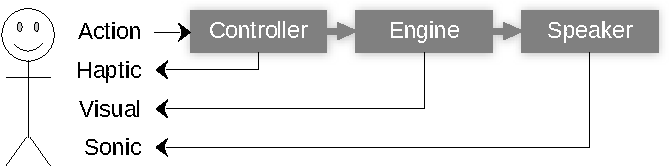
\includegraphics[width=0.9\columnwidth]{figures/48-feedback-crop.pdf}
	\caption{A sketch of three different types of feedback in an electro-acoustic instrument.}
	\label{fig:mapping-feedback}
\end{figure}

Visual feedback is another critical element of most electro-acoustic instruments, arguably more than in acoustic instruments. Such visual feedback can be in the form of light, for example, blinks or changing colors. Screens have also become prevalent in electro-acoustic instruments and are growing larger every day. In fact, in tablet-based and mobile phone-based instruments, the screen has taken over the entire interface. \citet{barbosa_direct_2019} argues that visual feedback needs to be direct, intuitive, and rapid. This helps compensate for the lack of physical feedback. The downside is that visual feedback makes it necessary to look at the instrument. This may potentially lead to communication challenges if the performer continuously stares at their instrument. Another problem with visual feedback is that it is often binary in nature. Many electro-acoustic instruments have lights that turn on and off to display whether some function is activated. This is a `cost-effective' feedback strategy that has the advantage of quickly giving the user control of many different types of parameters. The downside is that such feedback may tend to focus on displaying information about technical parameters. Having static binary feedback may also discourage continuous control.

The third feedback layer sketched in Figure~\ref{fig:mapping-feedback}, is that of haptic feedback from the controller. Many electro-acoustic instruments have a mechanical interface, which may act back on the user. For example, the keyboard of an electro-acoustic instrument provides some tactile and haptic feedback in itself. Some high-end commercial instruments, like digital pianos, have active haptic feedback, and we will look at one such example in Chapter~\ref{chapter:conventional}. The interest in haptic interfaces has increased rapidly in the music technology research community \citep{papetti_musical_2018}, so I expect more of this feedback modality in the years to come.

\citet{braasch_telematic_2009} reflects on the complete neglect of \emph{olfaction} in musical instrument designs. The sense of smell is much older than many other modalities from an evolutionary point of view but is rarely used in human-computer interaction. This is not only about digital scent technology; the smell of an instrument is primarily related to its physical materials. As for most other technologies, metal and plastic have dominated the construction of electro-acoustic instruments. There are some examples of the usage of other materials. Wood has seen a revival, and there are also examples of the use of leather in instruments \citep{favilla_bent_2005}. This certainly helps in creating a richer olfactory (and tactile) experience.

While there may be exceptions, I would argue that an instrument's feedback level is directly linked to its experienced action--sound separation. Feedback is something you get for `free' in acoustic instruments, particularly those with a smaller separation between action and sound. On the other hand, each feedback layer needs to be designed and constructed in electro-acoustic instruments. The larger the action--sound separation of the instrument's construction, the more focus needs to be put on creating feedback. A good example here is the visual feedback design of the `buttons' of the Ocarina mobile phone-based instrument. \citet{wang_artful_2018} describes how carefully these were designed, with many visual layers, each having a different purpose. Such detailed designs are essential when the rest of the action--sound chain may be sub-optimal. Then multimodal feedback may be used as a way of improving the overall experience of the instrument.


\section{Action--sound separation}

Since the construction of electro-acoustic instruments is fundamentally different from acoustic instruments, I do not think it is possible to use the same categories when talking about an instrument's action--sound separation. I will instead propose six categories that are more focused on the type of mapping process involved:

\begin{description}
	\item[Embodied:] The body is directly involved in the sound-production or modification, such as in the Theremin or Cracklebox.
	\item[Analog:] There are continuous (electric) relationships between action and sound, like in most analog synthesizers.
	\item[Digital:] There are discrete (sampling-based) relationships between a physical input device and controller.
	\item[Virtual:] There are multi-layer relationships between action and sound, such as in apps and web-based instruments.
	\item[Automatic:] The instrument can play on its own.
	\item[Conceptual:] There is no physical instrument to interact with; the instrument and its sound-production are only happening within your (embodied) mind.
\end{description}

These can be laid out schematically (Figure~\ref{fig:electroacoustic9}), referring to whether there is a tighter or more loose action--sound separation. In the following, we will look more closely at each of these categories before discussing some more complex examples.

\begin{figure}[tbp]
	\centerline{
		  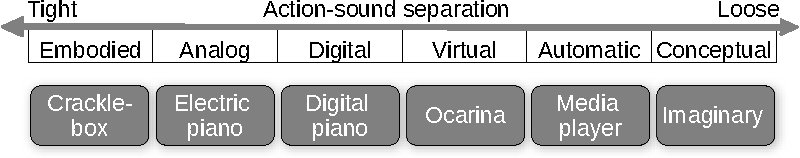
\includegraphics[width=\textwidth]{figures/49-separation-crop.pdf}
			\caption{A sketch of different types of action--sound separation found in electro-acoustic instruments.}
			\label{fig:electroacoustic9}
}
\end{figure}


\subsection{Embodied instruments}

Are there any electrically-based embodied instruments? No, if we think about embodied acoustic instruments such as the voice. Here we will also leave out hybrid instruments based on amplifying body sounds in one way or another. Still, some electro-acoustic instruments are more embodied than others.
The Theremin is one of these, played by moving the hands within the range of two metal antennas. One of the antennas controls the frequency of the sound, and the other the amplitude. It may seem like a contradiction to call the Theremin an embodied instrument, while at the same time, it is also one of the earliest analog instruments and the first `touchless' instrument. However, the presence of the performer's body is necessary to both produce and modify the sound. When considering the whole chain from action to sound, I find it interesting that the original Theremins were constructed with a built-in speaker. In modern-day versions of the instrument, the speaker has been removed.

Another instrument that could be considered partly embodied is the Cracklebox (Figure~\ref{fig:Cracklebox}). This instrument was invented by Michel Waisvisz at STEIM in Amsterdam in the 1970s. Its construction is based on a single operational amplifier and a few transistors. The box has six metal contacts on top, and sound is produced when the performer touches the metal contacts to shortcut the circuit. The human body becomes a part of the circuit and determines the range of possible sounds. The sound comes from a small speaker in the box, so the Cracklebox is a complete electro-acoustic instrument.

\begin{figure}[tbp]
	\centering
		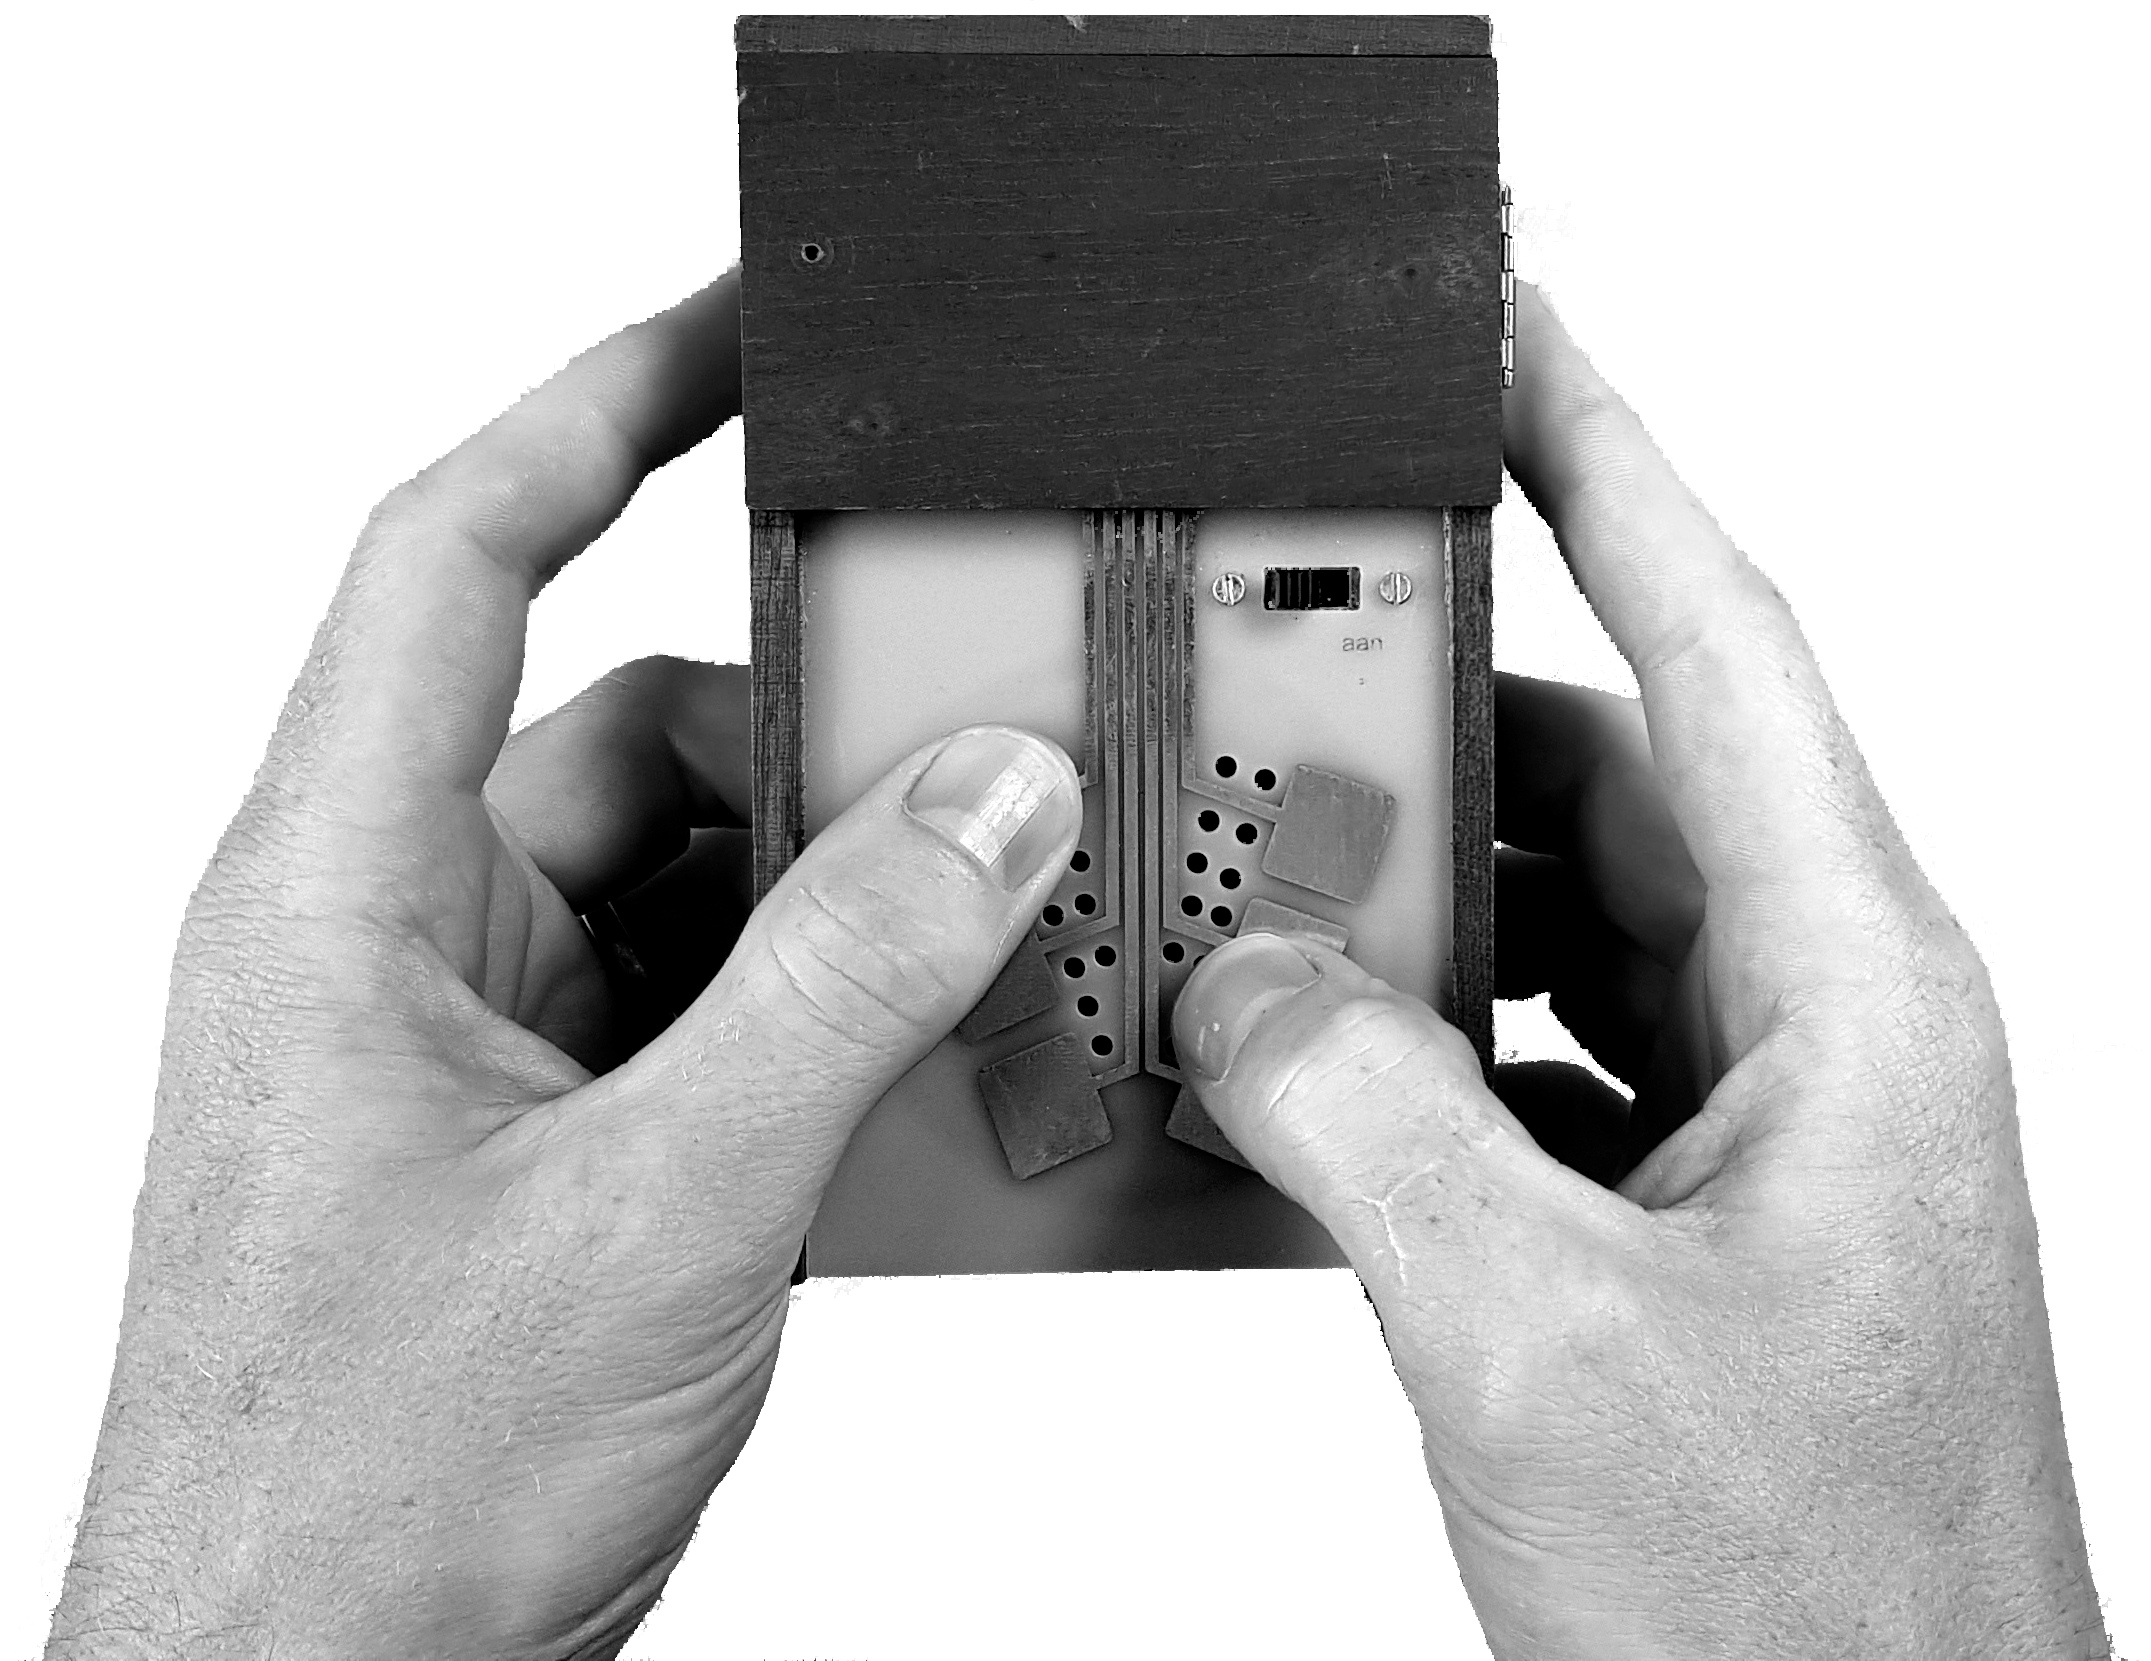
\includegraphics[width=0.7\columnwidth]{figures/50-cracklebox.jpg}
	\caption{A Cracklebox is played by touching the metal contacts on the top, thereby shortcutting the circuit to produce sound.}
	\label{fig:Cracklebox}
\end{figure}

\citet{waisvisz_crackle_2004} describes the invention of the Cracklebox as inspired by touching the inside of his father's short-wave radio receivers. This resulted in alterations of the sound, through which he could start to play directly with the sound waves. From my action--sound perspective, I find it fascinating to read the reflections of \citet{waisvisz_crackle_2004} on the physicality of the Cracklebox:

\begin{quotation}
Finger pressure curves are very basic information standards. The act of applying physical effort through touch is empirically `known' to all human beings. The listener can feel the performer's touch and recognize the effort. The handling of physical effort is part of a universal language.
\end{quotation}

I find Cracklebox an inspiring instrument, mainly because it is unpredictable. When first touching it, you may not get any sound at all, particularly if you have dry fingers. It relies on some sweat or moisture to be conductive. The next challenge is to make consistent sonic results. I often find myself sitting with it for long periods, exploring new types of `sonic shapes.' The timbral quality of the sounds is usually not that interesting; however, the close relationship between finger action and sound results in human-like sonic shapes. I also like that the Cracklebox has a built-in speaker. This creates an immediate connection to the sound being produced, further strengthened by the zero-latency of the simple analog circuit. The use of wood and metal in the construction additionally helps create the feeling that you are playing a `real' instrument, not just a toy. It may be the combination of all these factors---the tactility, performability, and playfulness---that together make for what I will later describe as an \emph{affective} experience.


\subsection{Analog instruments}

Analog electro-acoustic instruments come in all sorts of shapes, sizes, and levels of complexity. I mentioned the Theremin and Cracklebox as partly embodied instruments, but they are certainly examples of analog instruments. Another of my favorite analog instruments is, in fact, even simpler: the Victorian synthesizer \citep{collins_handmade_2009}. This is one of a few genuinely \emph{electric} instruments since there is no electronic circuit involved. It contains so few parts that everyone can build it themselves. It only consists of a battery, a speaker element, and cables connecting them, shown in Figure~\ref{fig:victorian-synthesizer}. Sound is produced when the circuit is closed between the battery and the speaker element. This creates a single `spike' of sound and immediately invites further sonic exploration. There is no latency in the chain, and you can feel the vibration in the speaker element when it happens, so there is both sonic and haptic feedback provided to the user. It is possible to develop small self-playing music machines by adding more speakers, cables, and extra metal pieces into the chain (paper clips work great, for example). I find the Victorian synthesizer to be excellent in teaching principles of sound technology. It demonstrates the core elements of an electro-acoustic instrument, and literally, everyone can make it work. With some practice, it is even possible to come up with relatively complex musical results. I once had a group of students that managed to create a sophisticated rhythmic structure by connecting the various parts I had given them in class.

\begin{figure}[tbp]
	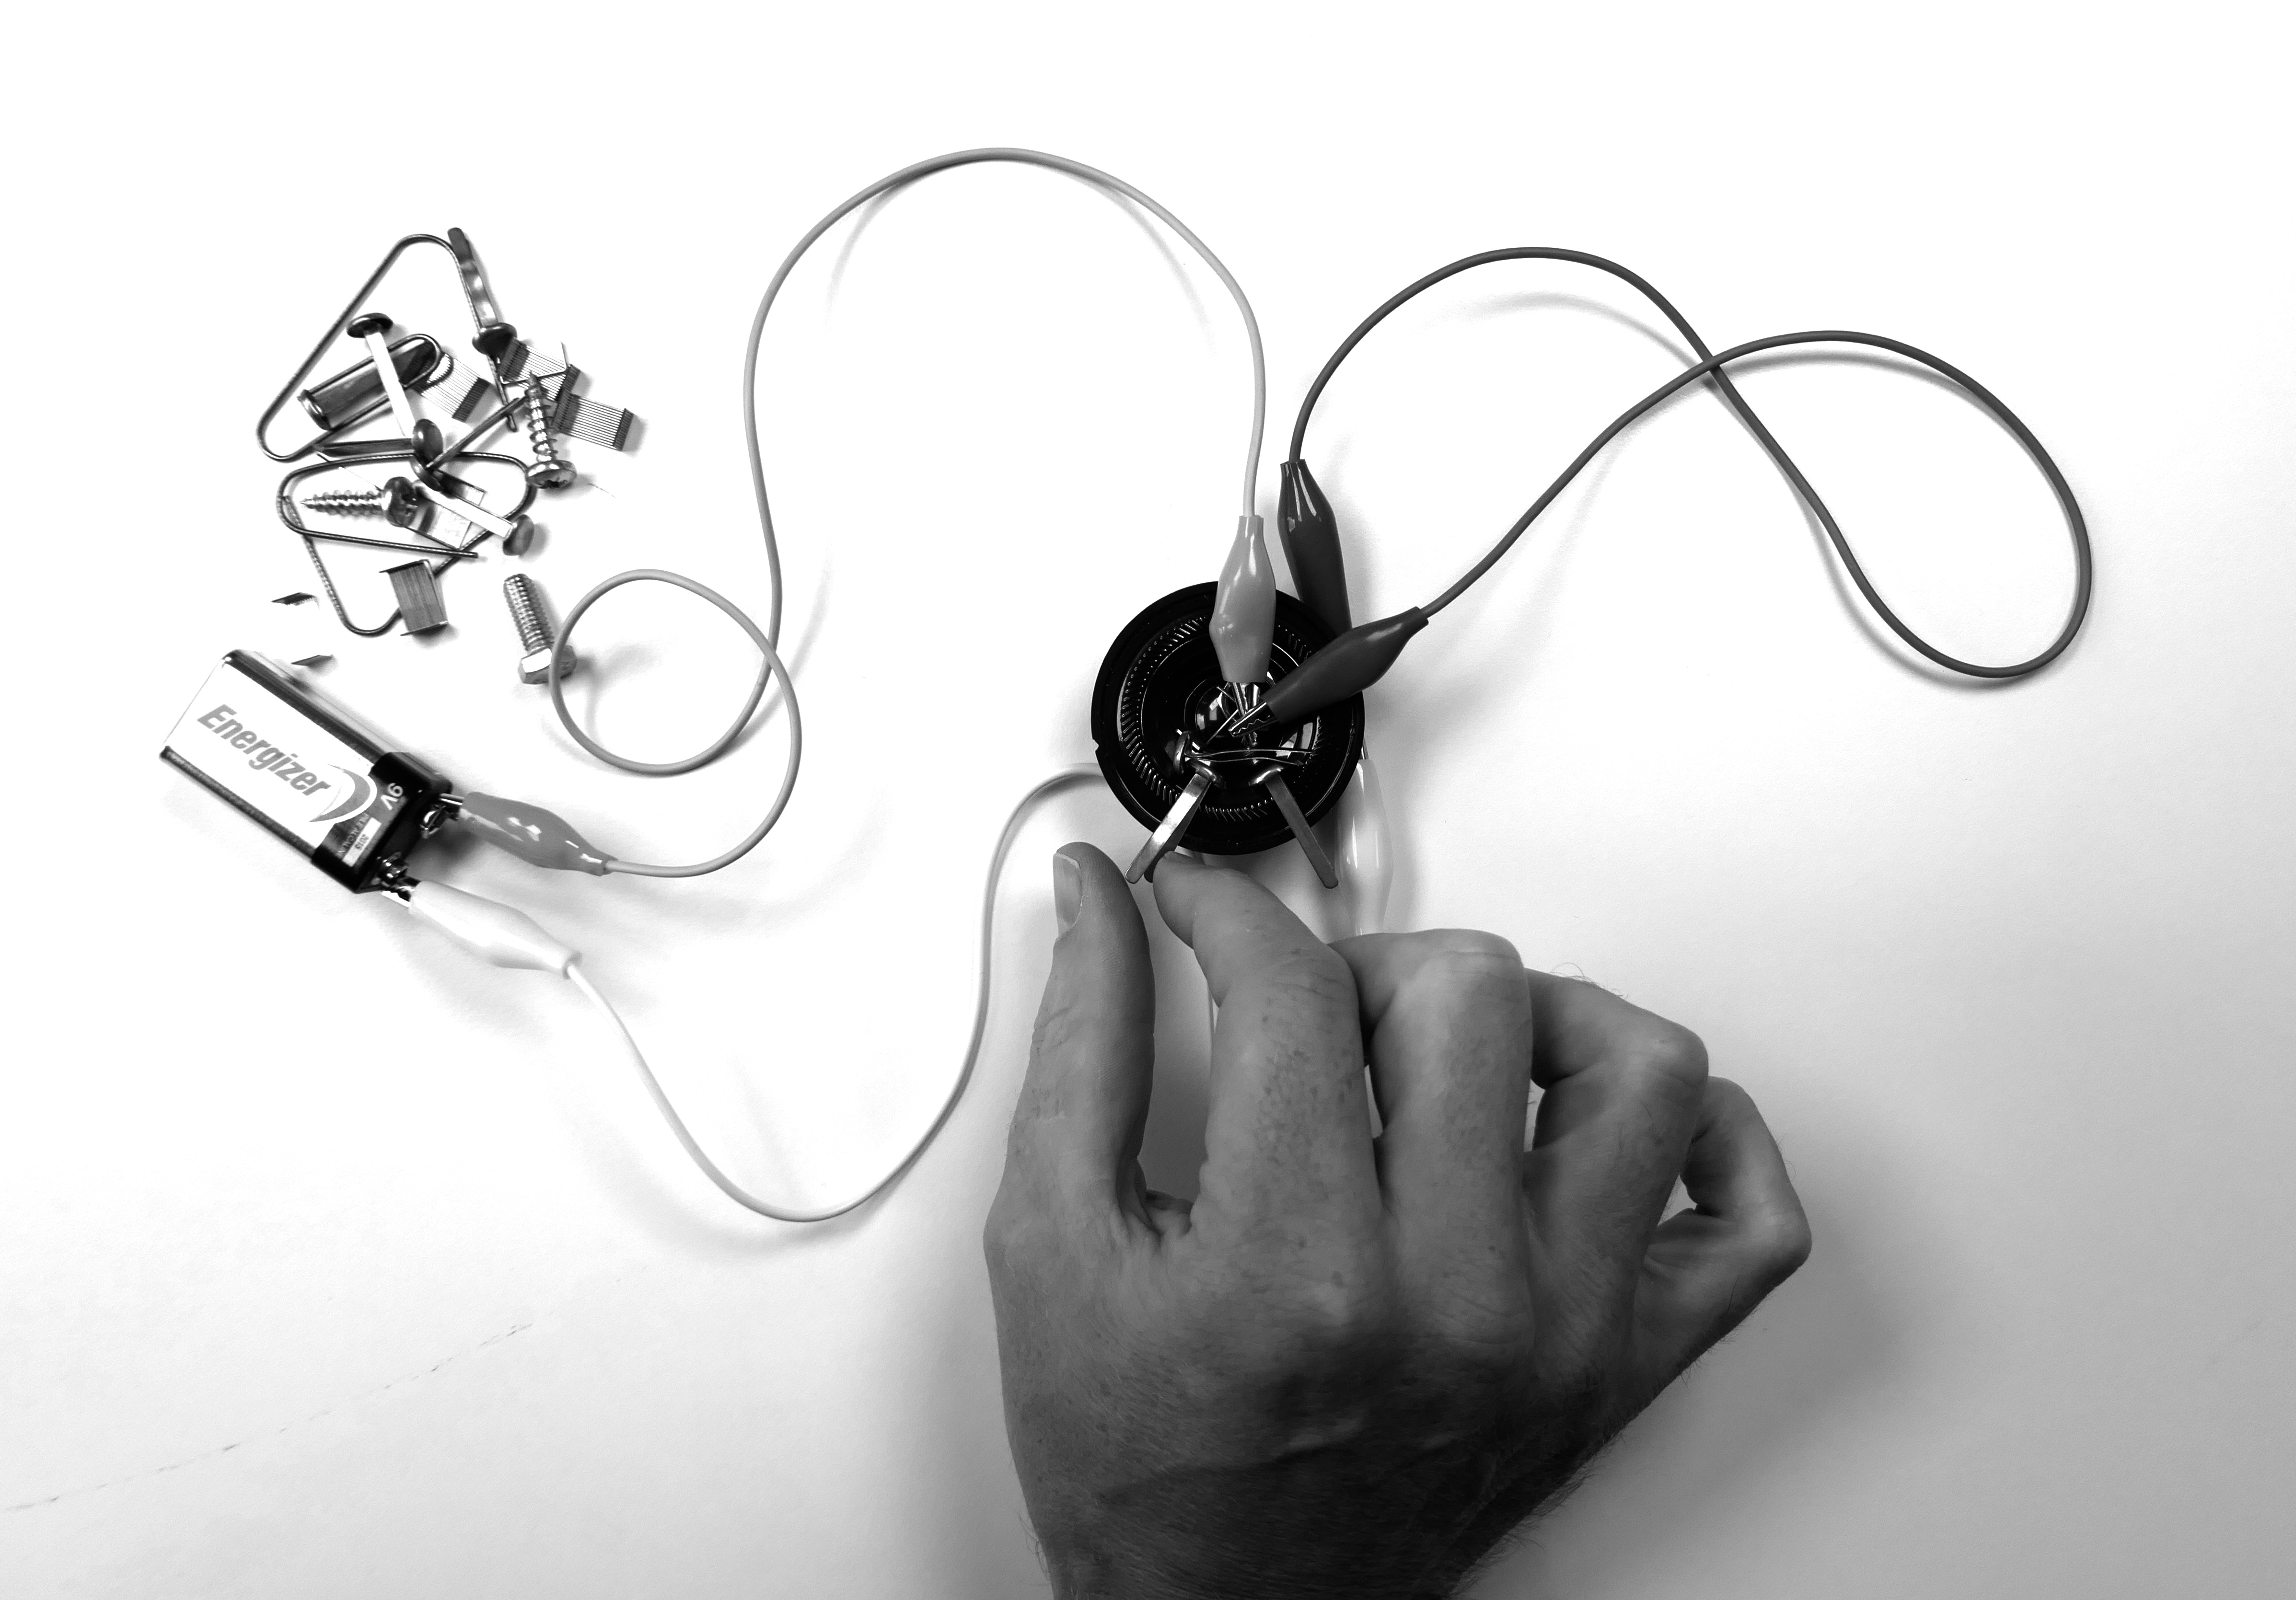
\includegraphics[width=1\columnwidth]{figures/51-victorian.jpg}
			\caption{A Victorian Synthesizer is possibly the most simplistic electric instrument. It only contains a speaker element, a battery, and cables between them. The instrument can be played by adding metal pieces to the circuit.}
			\label{fig:victorian-synthesizer}
\end{figure}

There are numerous examples of more complex analog instruments; see, for example, the excellent overview of analog synthesizers by \citet{jenkins_analog_2007}. When browsing catalogs of commercially available analog instruments, one realizes that the keyboard quickly made its appearance. Famous examples of early analog instruments---such as the Ondes Martenot---rely on a piano-like control surface. As we know, keyboard-based control has remained remarkably popular in later generations of analog instruments and has also been the de facto standard in digital interfaces. Of commercially successful instruments with keyboard control, one could mention the Hammond organ, Wurlitzer piano, and Moog synthesizers. I find it interesting that while the Hammond and Wurlitzer are often referred to as `organ' and `piano,' respectively, many Moog instruments are called `synthesizers.' This may be seen as part of the shift of attention from instruments being sound-makers to music-makers. Many of the early synthesizers could be thought of as something in between: `sound-modifiers.'

It is also worthwhile reflecting on the use of the term `keyboard.' The word itself refers to the controller of an instrument, as you would find in a piano or organ. Synthesizers, however, come in all shapes and do not necessarily need to have a keyboard-like controller. So what is the difference between playing a `synthesizer' and playing a `keyboard'? I have heard people argue that the main difference is that synthesizers do not have speakers built-in, while keyboards do. The same people may also disregard such keyboards as toys for kids. In my thinking, the two terms are incomparable. One describes the controller (keyboard), while the other the sound engine (synthesizer). Numerous instruments with a synthesizer as a sound engine are not controlled with a keyboard interface. There are also examples of keyboard-based instruments that are not based on sound synthesis, such as sample-based devices. Nowadays, it is also common to buy keyboard controllers with no sound engine nor speakers.

The gradual modularization of electro-acoustic instruments---both analog and digital--has changed how music is made. The first analog devices were standalone instruments, complete with a control interface, sound engine, and built-in speaker. Then the speakers were `removed,' before also the controller was split from the sound engine. Finally, the sound engines were split into many small components.
This gradual modularization was at least partly driven by the ability to route control voltage signals in different ways \citep{bjorn_patch_2018}.
With an increased standardization among manufacturers, it became possible to send electric control messages between devices. The development of digital MIDI signaling, reduced the need for passing electric signals between devices. Analog instruments also saw a general decline after the introduction of digital devices in the 1980s. Still, analog devices kept being developed and used, and we have recently witnessed a revival \citep{barlindhaug_kids_2019}. Several manufacturers have taken up production of old analog models or developed affordable versions of old synthesizer concepts. There is also a growing interest in modular, analog synthesizers made accessible by the standardization into Eurorack modules. Also, the `circuit bending' communities have embraced using and modifying analog electronics for musical applications \citep{skjulstad_circuit_2016}. So analog electro-acoustic instruments are here to stay.

As we are getting to the end of this section on analog instruments, some readers may wonder why I left the electric guitar out of this discussion. That is because I am thinking of the electric guitar as a hybrid instrument, based on the amplification of an \emph{acoustic} instrument. We will return to a discussion of the electric guitar and other hybrid instruments in Chapter~\ref{chap:hybrid}.


\subsection{Digital instruments}

Digital electro-acoustic instruments differ from analog in that they are based on a discretized signal chain. This is done by using ADCs to convert control signals into a digital representation and the use of DACs to convert digital signals into audible sound. In my taxonomy, I separate \emph{digital} and \emph{virtual} instruments. This may seem like an arbitrary division, but the idea is to consider devices that have some kind of mechanical controller (such as a physical keyboard) separately from devices played through an intermediary control layer (such as a touch screen).

Digital instruments were gradually introduced to the market in the 1980s, with the Yamaha DX7 being the first commercially successful digital synthesizer \citep{shepard_refining_2013}. The possibilities of digital instruments have increased rapidly. What has remained remarkably constant, however, are the controllers. Even though we see some new explorations into multi-touch controllers, most commercial devices still rely on keyboards and variations of the `knobs-and-sliders' paradigm. The conservatism of manufacturers may (at least partly) be explained by the limitations of the MIDI standard. As discussed in Chapter~\ref{sect:midi}, the note-on/note-off type messaging is designed for keyboard-based instruments, and the control message paradigm lends itself well for control by buttons and knobs. When there is a whole technological ecosystem built around this standard---which works well in many ways---it is challenging to think anew.

One of the benefits of MIDI is that it allows for modularizing setups. This modularization began with analog instruments and has become more prevalent in the world of digital instruments. On the positive side, one can use multiple sound engines with one controller or numerous controllers with one sound engine. However, this flexibility often leads to more complexity and difficulties in getting things to work. I have spent countless hours reading manuals and fiddling with settings to pass signals from a controller to a sound engine. Setting up for a soundcheck is also much more time-consuming with modular setups than when using self-contained instruments. So the modularization has a downside when it comes to the level of `plug-and-playability' of instruments. It also leads to an increased action--sound separation, mainly when using different sound engines with the same controller.

In the taxonomy, I do not separate hardware-based and software-based digital instruments. One could argue that all digital devices are hardware-based since they have a computer inside. However, there are differences between instruments based on micro-controllers versus general-purpose PCs. For example, instruments built around micro-controllers can often be more efficient for the task at hand despite their inferior technological specifications. DSP-optimized chips and their single-purpose design can compensate for the lack of computing power in such embedded devices. That said, PC-based digital instruments have become so robust and powerful that they are currently used in many contexts.

Let us consider the setup of a typical `laptop musician.' This usually consists of a MIDI controller connected to a laptop running one or more music applications. The laptop is also connected to a sound card, passing the sound to a mixer and speaker system. Many things have improved in the world of computer music over the years, but I am unsure whether I spend more or less time troubleshooting my software-based instrument setups than my hardware-based ones. Computers usually give better error messages than hardware devices, but more things need to be connected to make the system work properly. Whenever I switch to a new laptop, I realize how many drivers and software packages need to be installed to get the different controllers and sound cards to work correctly. Constant software updates help fix bugs and add new features, but also lead to new problems and additional troubleshooting. Sometimes I am lucky and get things up and running quickly. However, I still think we are far from having true `plug-and-playability' in the world of laptop-based musicianship.

In addition to the `synthesizer-type' and `laptop-type' digital devices mentioned above, we should not forget about the digital instruments that aim to mimic acoustic instruments. In terms of sales numbers, I would guess that this is the largest category by far, of which digital pianos are probably the main driver. Several manufacturers have put in much effort to create instruments that are as `acoustic-like' as possible. This may be seen as an example of instruments that focus on decreasing the experienced action--sound separation and is something we will get back to in Chapter~\ref{chapter:conventional}.


\subsection{Virtual instruments}

Virtual instruments are also based on digital signal processing, so they could have been included in the category of digital instruments. Still, I think they differ from an action--sound point of view. A piano app on a mobile phone is an example of what I would call a virtual instrument. More precisely, it is not the app itself that is the instrument, but the app inside a physical phone with a touchscreen for input and a speaker for output. As such, a phone with a piano app is a complete instrument according to my definition. What makes such an app-based instrument different from a MIDI controller connected to a laptop is that there is one more abstract `layer' in the interaction: the app is played by touching `keys' on the screen. Thus the screen acts as a mediator between the finger and the virtual keyboard on the screen. Therefore, this interaction has one more degree of action--sound separation than a digital instrument in which you press on a physical key.

The same is true for web-based instruments, which you typically play by clicking with your mouse on `keys' in a browser window. Here the mouse is the physical interface, which is further mapped to clicking on the virtual key on the screen. Web-based instruments often also add an extra layer of abstraction on the sound-processing side. The Web Audio API has made it possible to develop powerful browser-based instruments \citep{smus_web_2013}. Many of these rely on sound-processing on the local machine. There are also examples of instruments in which all the sound-processing happens remotely. In some cases, even remote hardware devices can be controlled, such as in the network control of Joe Paradiso's modular analog synthesizer \citep{mayton_patchwork:_2012}. Both technologically and conceptually, this leads to a large action--sound separation. Such setups also create more latency than if all the processing would happen locally. The exception is whether the sound-processing is so heavy that it could not run in real-time on a local computer. Then there may be benefits of `outsourcing' the processing to a remote server that can perform in real-time, though slightly out-of-time.

While there are certainly some challenges regarding the increasing action--sound separation in virtual instruments, there are also several benefits. Server-based instruments may be more accessible to many people. There is no need for particular hardware on the user side; hence, users can start making sound without having to set up and configure anything. Large servers may also do much heavier processing than what could be done on a regular PC; thus, the final output sound could be more complex. However, the most interesting with server-based instruments may be the ability to engage in entirely new forms of musicking. \citet{wang_artful_2018} writes about the popularity of Ocarina, one of the first iPhone instruments. The sound-making part of Ocarina is clever. The microphone is used to pick up the user's breath and is used for sound production. The sound modification is done by touching virtual buttons on the screen. However, the most exciting part of the instrument is its ability to connect to a global community of other Ocarina players. This brings in a new social dimension and allows for large-scale collaborative musicking.

The Ocarina is an excellent example of a virtual instrument that embraces the possibilities afforded by new technologies. Many other virtual instruments are more focused on recreating the past. Just in the same way that we have seen a lot of digital instruments that imitate acoustic instruments, we now see a lot of virtual instruments that mimic analog and digital instruments. There are virtual versions of old analog synthesizers, with the complete looks and functionality of the hardware device. Instead of patching physical cables or touching knobs, the user controls the devices with a mouse or a touch screen. I find this somewhat peculiar. It is interesting from historical and educational perspectives, but I am more interested in developing and using new paradigms with new technologies than in recreating the past.

Another example of an innovative virtual instrument is Bloom by Brian Eno. This is also an iPhone-based app in which the user creates sound by tapping on the screen. \citet{eno_bloom_2008} describe the instrument as:

\begin{quote}
	[\ldots] an endless music machine, a music box for the 21st century. You can play it, or you can watch it play itself.
\end{quote}

The two modes of Bloom allow for different levels of musicking. When started in `playback mode,' it can be considered a self-playing instrument, similar to a music box. The `performance mode' allows for direct control of the tones being played. Here the user can touch the screen to control the pitch of the tones. So there is a clear and immediate control of individual tones. The underlying sequencer will repeat the same tones after a few seconds, and the user can add new tones to the mix. The user can switch between different settings, in which the scales and colors will change, but they are all laid out so that the instrument will always sound `nice.' I still remember my then one-year-old daughter's fascination as she pressed the screen and listened to the sounds. It both gave a sense of being in control (performing) and experiencing (perceiving). As such, Bloom shows how the traditional roles of musicking are in play. This was also Eno's intention, describing it as creating `gardening' experiences \citep{clark_estes_first_2018}:

\begin{quote}
	Imagine if composing could be more like gardening than architecture [\ldots] You do control the input, but you don’t control the output.
\end{quote}

While Bloom was primarily developed for individual usage, we enjoyed using it in performances with the Oslo Mobile Orchestra. As shown in Figure~\ref{fig:olo-verdikt}, this ensemble was based on performing in the tradition of a `marching band,' similar to other mobile phone orchestras \citep{oh_evolving_2010}. Each performer had a mobile phone, which was connected to a hand-held speaker. This made it possible to freely move around in the room while keeping a sound source close to the performer and giving the audience a spatial experience of the sound. Each mobile phone speaker was not particularly powerful, but having many of them spread around a space resulted in a submerged auditory experience. When it came to controlling the instrument, Bloom is so easy to play that I could teach the concept to new ensemble members in minutes. One person that performed with us in a concert once objected that this was not a `real' performance. She argued that only practicing for five minutes before going on stage was an example of `fake' musicianship. Yes, playing a concert with Bloom is different from playing a classical violin quartet piece. The exciting thing, however, was that audiences were thrilled about our mobile phone concerts. I have never gotten more performance requests than with that ensemble. So what we think of as `true' performance, and what people find musically interesting, may not always be the same.

\begin{figure}[tbp]
	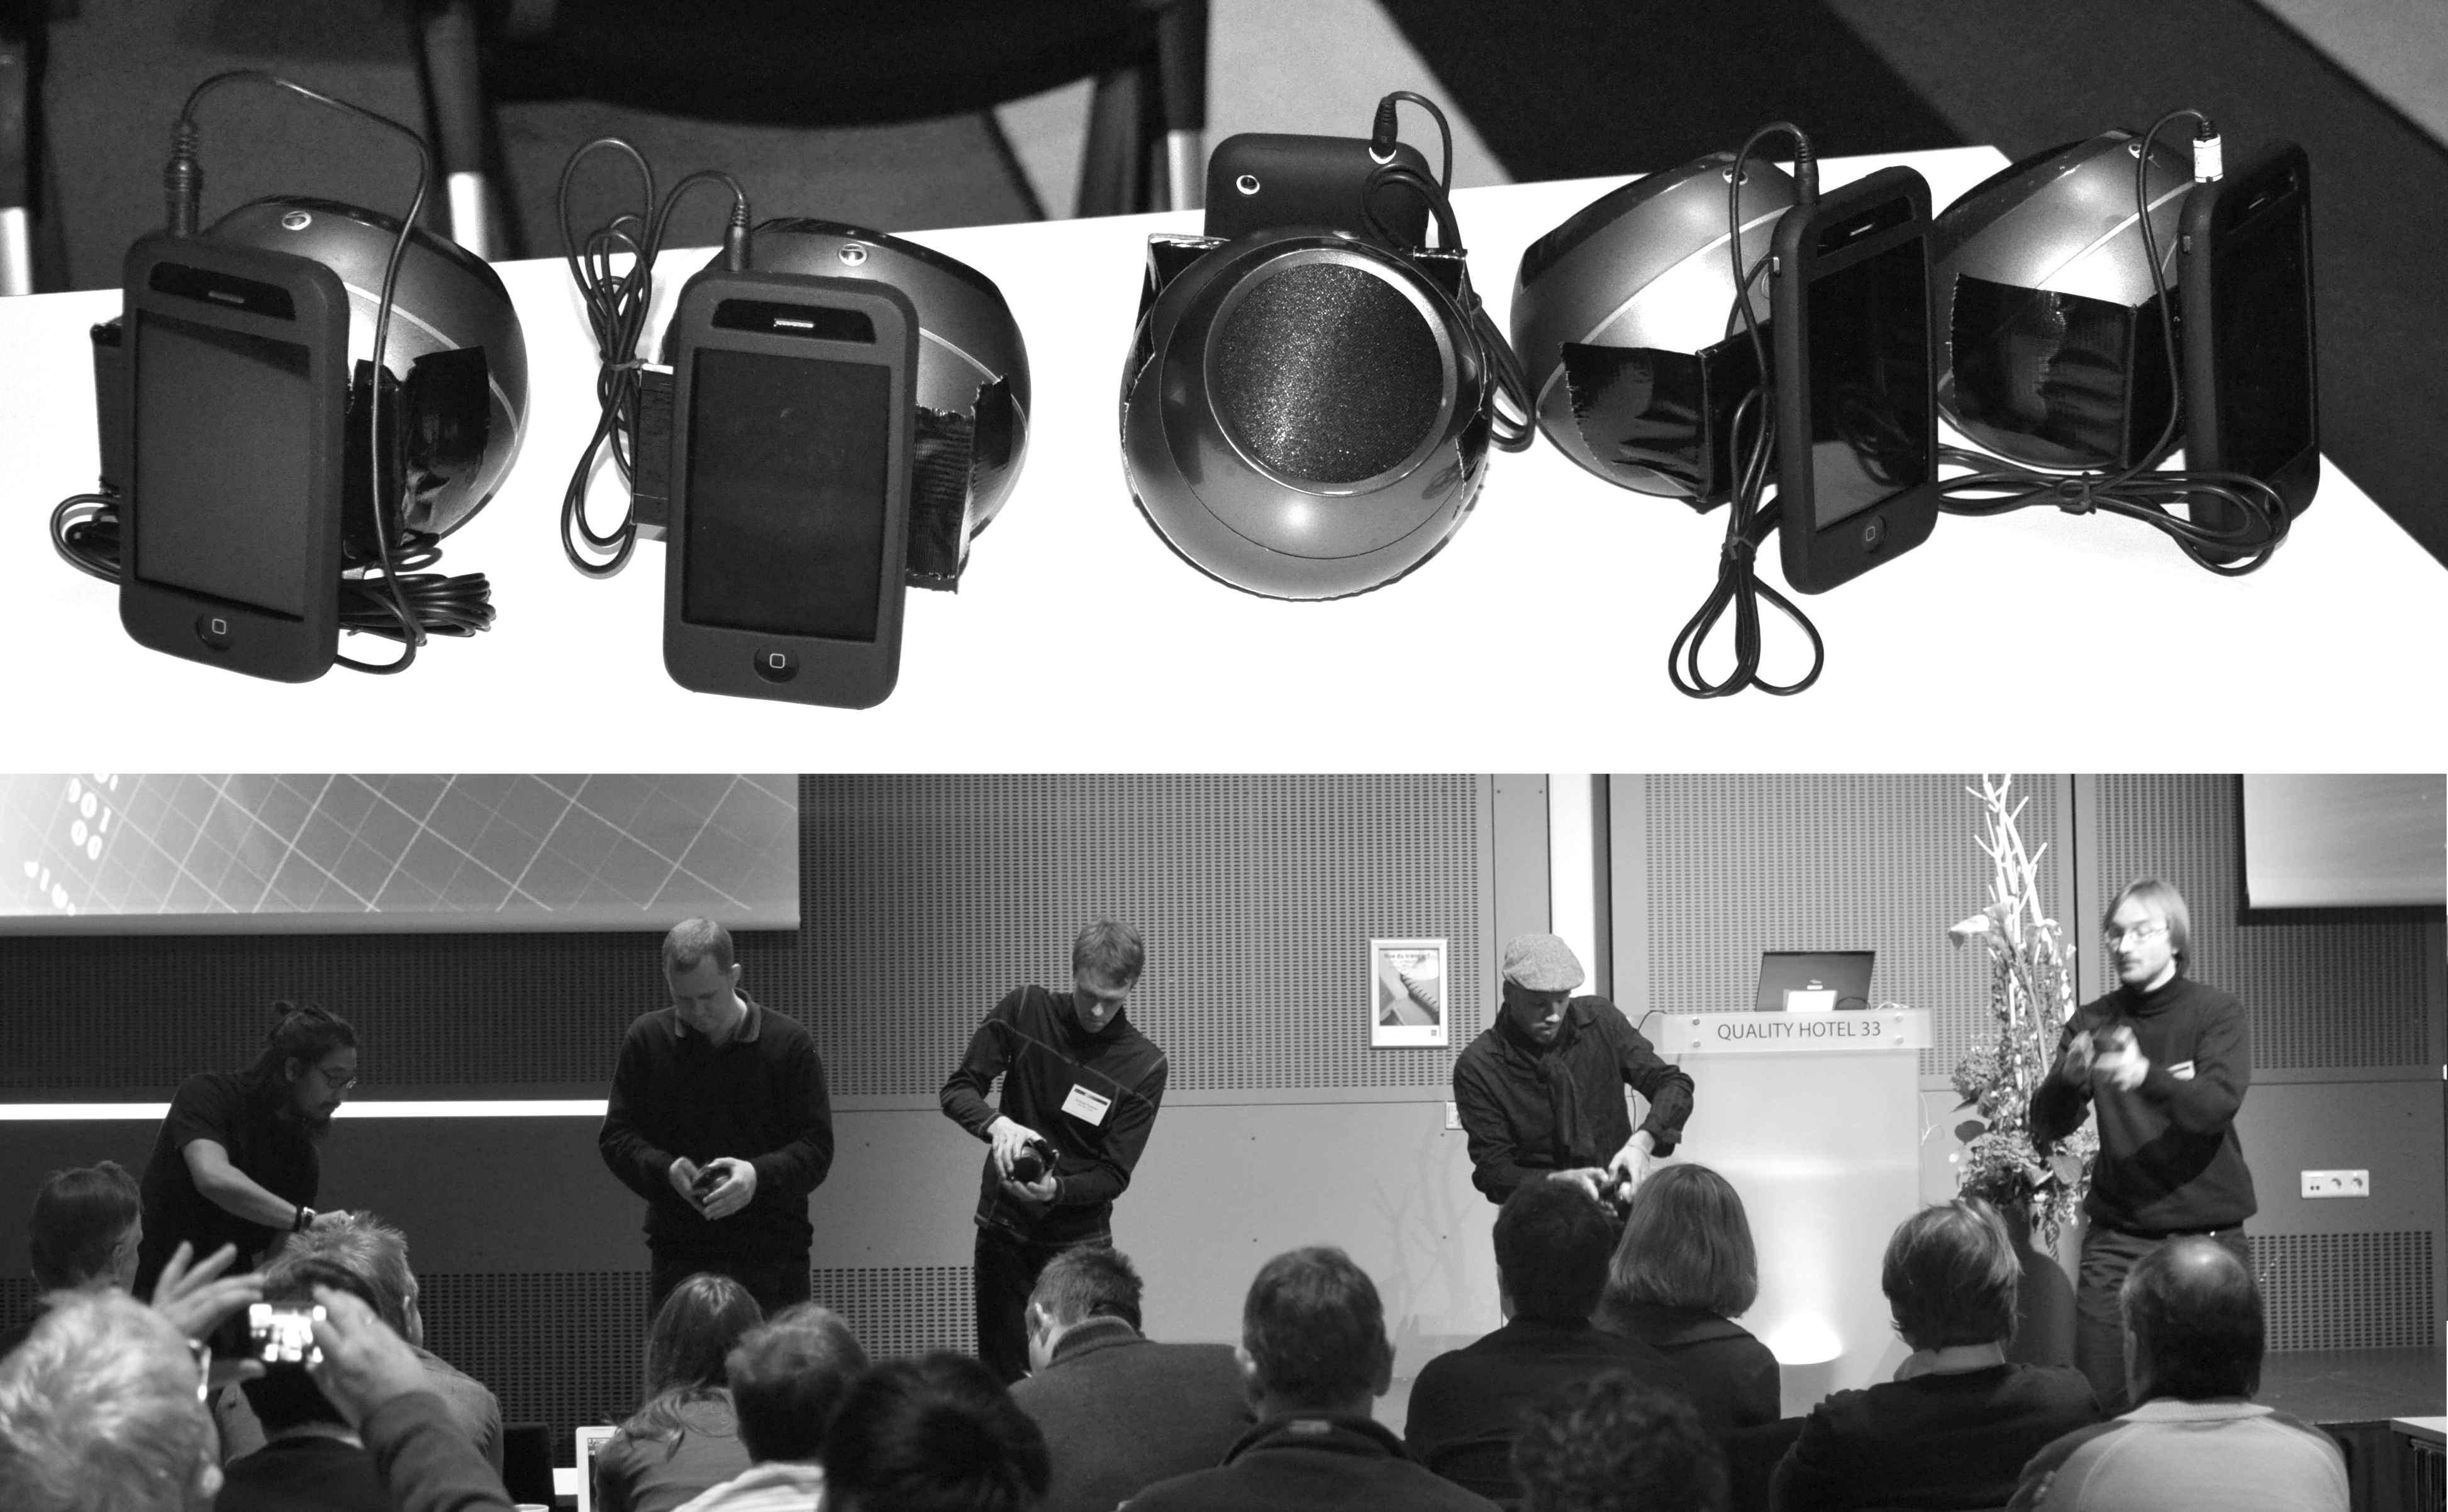
\includegraphics[width=1\columnwidth]{figures/52-mobile-orchestra.jpg}
			\caption{The Oslo Mobile Orchestra performing a piece using the performance-mode of Brian Eno's Bloom (bottom) (Photo: Ståle A. Skogstad). Each performer used a mobile phone connected to a handheld speaker (top).}
			\label{fig:olo-verdikt}
\end{figure}

\subsection{Automatic instruments}

Only a few acoustic instruments can play on their own, but most electro-acoustic instruments can. For example, most digital keyboards have a `demo mode' where you can listen to different tunes stored in the instrument. I still have fond memories of the demo songs on my first keyboard from the 1980s. To my parents' despair, I used to play these songs over and over as a child. That particular instrument is now at our family cabin, and my daughters are the ones to keep pushing the `demo mode' button while dancing to the tunes.

While automatic playback is possible on many electro-acoustic instruments, it is primarily an add-on feature to demonstrate their capabilities. Their initial design is still meant for being played by humans. Other instruments are made primarily for automatic performance. The playback mode of Bloom, for example, was intentionally designed as such. But also Bloom's performance mode could be considered a combination of virtual and automatic instruments, or perhaps more as an \emph{active listening} device. What is becoming tricky from a classification perspective, then, is to what extent music recording and playback devices should be considered instruments or not?

As described in the previous chapter, there are numerous examples of automatic acoustic instruments. These instruments were mechanical at first but then eventually became electrified. Without covering the whole story of recorded music---there are many excellent resources on that, such as those by \citet{wurtzler_electric_2007,katz_capturing_2010,devine_decomposed_2019} to name just a few---the 20th century saw an incredible development from the first player pianos to gramophones with wax rolls followed by the LP, cassette, CD, and MP3 players, and leading up to today's variety of streaming-based devices. These music storage devices are based on different technologies, but they share the same function of allowing for playing back recorded music.

In a review of musical agency in human--computer interaction, \citet{tatar_musical_2019} propose a taxonomy from \emph{purely reactive} agents on one side to \emph{completely autonomous} on the other. The autonomous instruments are arguably the most extreme case of automatic instruments. A former colleague of mine, Risto \citet[p. i]{holopainen_self-organised_2012}, defined these as:

\begin{quote}
	[\ldots] computer programmes that generate music algorithmically and without real-time interaction, from the waveform level up to the large scale form.
\end{quote}

He has continued to explore such instruments in both his research and composition practice. In the most extreme case, the computer can be programmed to create an instrument on its own, compose a piece for the instrument, play it back, listen to its creation, evaluate it, and use its aesthetic logic to reiterate and develop new instruments and music. While this may seem a bit far-fetched, we will probably see more examples of autonomous instruments playing what \citet{harper_infinite_2011} calls \emph{infinite music}.

I often hear people talk about autonomous instruments as synonymous with instruments driven by artificial intelligence (AI). An autonomous instrument could be based on advanced machine learning, but it could also be based on rule-based algorithms. If one argues that the latter should be considered AI, then autonomous instruments could be considered AI-based instruments. However, there are also cases where AI is used in musical instruments without them being autonomous. There may be machine learning algorithms on the sensing side, clustering algorithms in the sound engine, and evolutionary algorithms in the melody generator. Still, the instrument could be controlled by a human. See, for example, all the different approaches presented in \citet{miranda_handbook_2021} to get an overview of the current state of AI-based musicianship.

Autonomous instruments may seem like the ultimate example of a complete action--sound separation. However, using such instruments could also be an efficient way of generating musical ideas that could serve as a creative starting point for human musicians. Drum machines and accompaniment systems have been available for decades. Today's autonomous instruments are building on such systems and pushing them some steps further. Some people are afraid that AI-based instruments will take over the jobs of composers and musicians. What is clear is that AI has already entered most parts of the music world and will continue to develop in many directions. I see this more as an opportunity than a threat. Someone needs to develop the underlying algorithms and put them to use. This requires new types of musical knowledge and experience. Instrument makers, composers, producers, and performers are an important part of the transition to tomorrow's musicking.


\subsection{Conceptual instruments}

Some of the most extreme cases of autonomous instruments could perhaps also be considered conceptual instruments. In addition comes purely imaginary electro-acoustic instruments. They can also give rise to vivid musical imagery. In some cases, they can even be built. That is easier for electro-acoustic instruments, in which mappings can be created at will. \citet{lepri_fictional_2019} describe an experiment in which people were asked to create fictional, non-sound-producing instruments. Mockups of these instruments were later used to study how the designs could tell about the musical background of the inventor.

One example of an instrument that is both real and imaginary at the same time is \emph{Volume 3: Everything You Love Will One Day Be Taken From You} by Yann \citet{seznec_book_2019}. This is the third volume of a set of three instruments called \emph{The Book of Knowledge of Impractical Musical Devices}, inspired by the 13th-century \emph{Book of Knowledge of Ingenious Mechanical Devices} by Ibn al-Razzaz al-Jazari. Seznec set forth to create three instruments shaped like books and that, in various ways, play with our understanding of time, space, and sound. In the third book, he explores the concept of the degradation of sound. It is inspired by Alvin Lucier's \emph{I'm sitting in a room} from 1969. In the piece, Lucier recorded his voice and played it back multiple times in a reverberant space \citep{hasse_i_2012}. Each playback and recording led to changes in the sound, based on the strengthening of the resonant frequencies in the room. At the end of the piece, one can only barely recognize the rhythm of the original speech; all the frequency content has been disturbed. Seznec's instrument is playing with the same idea in that the user only has one button to press. That button is playing back a sample, but at the same time, it is also replacing the same sample with a slightly distorted version of itself. So by listening to the sound, one will also gradually destroy it. The instrument exists as a digital instrument, although few people get to play it in person. For me, and most others, it is equally important as a conceptual instrument.


\section{Some considerations}

As the above discussion showed, creating a taxonomy that covers all sorts of electro-acoustic instruments is challenging. I have considered many different types, but there are also many open holes in my theory. Let us consider some borderline cases.


\subsection{The need for a speaker}

While my instrument definition is flexible in many ways, I am strict about the need for instruments to make sound. Therefore, it is necessary to consider the whole chain from action to sound when analyzing an instrument. That means that a sound engine, such as a synthesizer module, is not an instrument on its own. It needs a controller for capturing actions and transmitting control signals. It also requires a speaker to produce sound. Similarly, a MIDI controller is not an instrument on its own; it necessitates a sound engine and speaker. Furthermore, a speaker is not an instrument; it needs a controller and sound engine.

This way of thinking about an instrument may seem radical. For example, it means that all the `digital musical instruments' that rely on external speakers are not instruments on their own according to my definition. However, they can be considered as part of an instrument if we also count in the speaker. Then, it is possible to view the whole chain from action to sound, including cables and other necessary components to produce audible sound. If there is no speaker, there is no sound. If there is no sound, it cannot be heard by the performer or the perceiver. This is the same as having a violin without a bow and strings. The violin needs strings and a bow to produce sound and hence be considered an instrument.

Some people ask me why I am arguing so strongly for considering the whole chain from action to sound in instruments. They say that a DX7 will sound like a DX7 even if you connect it to different speaker systems. I agree that the DX7---and many other signature synthesizers---have unique sonic characteristics. Still, the final sounding sound depends on the speaker system used. Playing through headphones is not the same as playing through a Hi-Fi system at home or a PA system in a club. The playback method largely influences the resultant sound. I still remember when I connected my first digital piano to a large PA system. Until then, I had mainly played it at home with headphones. Using it on a stage with sound coming out of a PA system was an entirely different experience. In short, it felt like a new instrument.

Being strict about considering the whole chain from action to sound may feel limiting. However, it is also a way of acknowledging the complexities of today's and tomorrow's musicking. It is easy to define the instrument when one plays an acoustic guitar. The same is not the case with a laptop-based rig or a telematic performance setup. Many computer-based setups rely on a range of connected hardware and software components. If we want to understand how the music is performed and perceived, it is necessary to consider the whole chain from action to sound.


\subsection{Music playback devices}

Let us return to the question of how a music playback device---whether in the form of an LP player or a media player on a mobile phone---could be considered an instrument. In Chapter~\ref{sec:automatic} we discussed how a pianola or music box could be thought of as musical instruments, even though they are based on playing back pre-recorded musical material. Still, they are devices made for performing music in real-time, albeit with relatively few control parameters available for the user. Modern-day music playback devices are similar but allow for more control of the final music. They can start and stop the playback, move back and forth in a song, and control the loudness through an amplifier. In some cases, they may have rudimentary tone control through `treble' and `bass' buttons. Sometimes they may even have a built-in equalizer. All in all, these control possibilities allow the user to shape the final output considerably.

There are only slight differences between an old-school gramophone player and a modern LP player. One relies on mechanical power from a wound-up spring, the other runs on electric power. They both rely on discs with engraved musical information and a pickup that transforms the signal into audible sound. In my thinking, both gramophone and LP players can be thought of as musical instruments. In fact, LP players have been on stages for decades, in the hands of DJs. A typical DJ setup consists of two LP players, a mixer, a microphone, possibly some sound effects, a pair of headphones, and a PA system. Therefore, one may argue that for the DJ, it is the complete set of devices that make up the instrument. I also find it interesting that there are two sound-generating devices in a DJ setup: the headphones used by the performer to pre-check the tracks and the PA system from which the final mix is played.

DJs make a living from playing (with) pre-recorded music. Some create a playlist before a show, and the only thing they do in real-time is to start and stop the playback. One could argue that most of the musical choices and work of such a `playlist DJ' are done out-of-time and possibly in non-real-time with respect to the `now' of the performance. This resembles the role of a composer but could also be seen as somewhat similar to the way a conductor selects repertoire and controls the start/stop of the performance and sound levels. Other DJs are more active performers, selecting new tracks, carrying out sophisticated beat-matching, adding vocals, and performing elaborate `scratching' techniques. \citet{hansen_acoustics_2010} has shown how scratching has developed into a skillful performance practice with a complex musical output.

The most experimental DJs, who are often referred to as \emph{turntablists}, typically work with all sorts of mediums under their turntable stylus \citep{smith_hip-hop_2013,holmes_electronic_2016}. Here the LP player can be considered a particular type of `mic-and-amp' setup since the stylus effectively works as a contact microphone. Many people would probably agree that a turntablist is, indeed, a musician performing with an instrument. However, the instrument in question---the LP player with the sound system---is the same. As such, it is hard not to classify this as an instrument. It was, after all, even designed and made for making music. The same can be said about the new digital music playback systems that DJs commonly bring on stage. Just as for LP players, they also allow for various types of real-time music-making.

Many would probably agree that a DJ or a turntablist can be considered a musician. However, it is more radical to claim that everyone using such technologies is a musician. Are you a musician when you turn on music on your mobile phone? According to my definition, yes. A mobile phone with a pair of headphones can be considered a complete musical instrument. And if you start and stop the playback of music and adjust the volume, you are actively taking part in the music-making. You have limited degrees of freedom available for controlling the sound, but you are still in control of what is going on. You can skip songs, change the volume, and modify the sound settings. This is different from standing on a stage in front of many people, but the principle is the same: you \emph{music}. Whether you are a performer or perceiver is not about what you do but about the role you take on. The new technologies continue to blur these lines.


\subsection{The laptop as an instrument}

Many electro-acoustic instruments are based on a computer in one way or another, whether it is a small embedded device in a digital piano, a laptop in a PC-based setup, or a high-end server in an online instrument. \citet{kvifte_instruments_1989} reflects on the change of `computers' from being humans doing manual calculations to machines taking over the same work. In any case, today's machine-based computers run programs created by humans. So humans are still in control of the final output. In his discussion of \emph{machine musicianship}, \citet{rowe_interactive_1993} discusses the differences between score-driven and performance-driven systems. As mentioned in the previous chapter, a music box, pianola, or LP performance can be thought of as score-driven. On the other hand, a performance-driven system relies on the performer to make musical decisions.

Nowadays, laptops are ubiquitous for music-making and are, in many cases, part of an instrument. However, can a laptop be an instrument on its own? \citet{fiebrink_dont_2007} argue that laptops have several built-in controllers (keyboard and mouse-pad) and sensors (microphone, camera, tilt sensors, and light sensors). These can be used to control software-based sound engines. Laptops also have built-in speakers so that they can produce sound on their own. Laptops can even be considered mobile instruments since they can be moved around during performance. The same is the case with mobile phones and tablets, both of which can be considered complete musical instruments with relevant software installed. All of these devices---laptops, phones, tablets---fulfill my action--sound criterion: the ability to sense action and output audible sound. The same is not the case for a desktop PC, which needs to be connected to controllers and speakers to sense action and produce sound.

In our department, we have a growing number of students who reply with `laptop' when they are asked about what instrument they play. When someone tells me that they `laptop' I always ask about what type of setup they use. Then they usually come up with a long list of different types of controllers, sound cards, mixers, and so on. When I ask them whether all of these devices should be considered part of their instrument, they agree that everything should be included. So it turns out that the term `laptop' is just a short form of a more extensive setup. This is similar to how someone playing percussion would not list up all the different sound-producing devices they may bring on stage. However, few laptop musicians include a speaker in the description of what they play. Some do, usually those that play guitar together with their laptop. Electric guitarists often think about a particular guitar amp as part of their instrument. They tend to be concerned with how the guitar sound blends with the laptop sound.

What people use a laptop for in performance varies considerably. \citet{brown_computers_2012} suggests thinking of three types of usage of computers in music: as a \emph{tool}, as a \emph{medium}, and as an \emph{instrument}. Sound recording and processing are examples of how a computer is used as a tool. Listening to music streams would be a case of the computer as a medium. A typical laptop performance scenario would be considered an instrument. In my experience, these three categories tend to fuse in performance. As discussed above, a DJ may use the laptop primarily for playing back recorded music. A guitarist may use the laptop for playing some pre-programmed drum beats to improvise over. In other cases, a laptop may be used as a `looper' or to add effects. Finally, some may play the laptop as a `normal' instrument: real-time sound-production and sound-modification.


\subsection{Laptop orchestras}

The development of the laptop as a musical instrument also sparked off an interest in \emph{laptop orchestras}. While many had been using laptops in various performance constellations, the Princeton Laptop Orchestra (PLOrk) is often considered a forerunner in form and organization \citep{trueman_why_2007}.
The conceptual idea of modern-day laptop orchestras has been to explore the use of computer-based instruments in `classic' ensemble-based musicianship: trios, quartets, and even larger ensembles with tens of performers \citep{knotts_politics_2014}. These orchestras are often related to educational activities. They have the same hardware setup, including laptops, controllers, and speakers. I find it particularly interesting that so much focus is put on the speaker. This is perhaps the most distinguishing element of such laptop orchestras from other types of computer-based performance. The reason for this is that, just like in an ensemble based on acoustic instruments, the musicians need to hear their own sound and the other musicians' sound. This was---and to a large extent, still is, I think---a radically different way of thinking about the sound projection from computers. Rather than having all the sound come out of a large PA, a laptop orchestra's sound emanates from each musician's location. In the context of PLOrk and its sibling ensembles, this sound source would not only be in mono or stereo but projected from multi-channel hemispherical speakers. As \citet{jensenius_author_2017} argues, the ability to have local sound projection has turned out to be essential for the many different laptop orchestras developed over the years.

As laptop orchestras developed, so did the need for conductors and scores. In some cases, orchestras have worked with human conductors with experience from acoustic-based ensembles. However, due to the peculiarities of laptop-based instruments, conductors would often need to develop specific techniques for laptop orchestras. Using laptops on stage has also opened for exploring the role of co-conductorship among the musicians. Instead of having a centralized conductor role, musicians can use messaging systems to conduct each other. This can also be combined with, or wholly overtaken by, computer-based conductors. The experimentation with different types of conductors has developed hand in hand with new kinds of scores. Since laptop-based music is rarely note-based, it has been necessary to experiment with alternate scores. From an action--sound perspective, I find it interesting that many of these scores focus on performance actions (`move hand in a circle') or audible sound (`play bright sound'). In any case, they aim to provide an efficient representation of what will be played, either through representations on paper or dynamically presented on screens.

There had been computer-based ensembles also before the development of PLOrk-style laptop orchestras. However, the institutionalization of the new wave of ensembles helped establish the laptop as a viable instrument in many universities and conservatories. With complete and relatively easy-to-use individual setups, the structured approach to laptop performance has served as an entry point to computer-based performance for many music students. In many cases, such ensembles have also attracted non-music students, effectively acting as an interdisciplinary melting pot. This attests to the usefulness of computers in both traditional and untraditional musicking. The development of repertoire, performance technique, and audience expectations has also helped shape the understanding that laptop-based instruments have come to stay.

One of the challenges I have seen with laptop-based instruments---particularly within the context of laptop ensembles---is how to handle changes in action--sound mappings from piece to piece. The physical setup stays the same in most cases, but it is common to change the mappings between pieces. This may not necessarily be a problem. Dramatic changes of action--sound mappings can be used creatively. However, the new mappings need to be carefully introduced to the audience for such changes to work effectively. It also helps if the mappings are based on a logical relationship between action and sound. Several laptop orchestras use different types of `gestural controllers' in performance \citep{tsoukalas_l2orkmote_2018}. This adds a visual element to the performance. I also see that the development of new performance strategies within laptop orchestras has inspired the `gestural' vocabulary also for other types of laptop performance.


\subsection{Live coding}

Next to laptop orchestras, there is another trend that has appeared in computer-based performance over the last decades, namely that of \emph{live coding} \citep{collins_live_2003}. This is a particular type of \emph{algorithmic music} \citep{dean_oxford_2018}, in which the musician starts the performance with a blank page on the screen. Performances are based on writing code in real-time, often projected on a screen for everyone to follow. This makes it possible for the audience to see the code development and how it turns into sound. In a way, this relationship between visible code and audible sound could be seen as the action--sound mapping in such a setup. A relevant question, however, is whether live coding can be considered an instrument? If so, I think it should be a virtual one since there are usually several layers of abstraction between action and sound. I would instead believe that it is the computer connected to a sound system that is the instrument. The code is part of the instrument but not an instrument on its own.

I am always fascinated by live coding performances. In many ways, it is a performance style that allows for seeing the performer's way of thinking about the generation of sound and musical structure before hearing the sound. As such, it may be thought of what \citet{chadabe_electric_1997} refers to as the real-time equivalent of algorithmic composition. However, the question about how such a performance relates to the `now' is tricky. Sometimes there is an almost immediate sonic effect of the code being written. This could be seen as an in-time performance. Other times it can take seconds (or even minutes) before the written code materializes in sound. Such out-of-time performance can be an efficient way of creating expectations. The use of countdown messages, for example, is particularly fascinating because it shapes the performance. A statement such as `kill all in 60 seconds' creates an expectation of what will happen. Even though many in the audience may not understand everything happening in the code, such clear messages can be understood by everyone and help structure the performance. This is why many people who usually would not care much about electro-acoustic musicking can find live coding fascinating.

Live coding is yet another example of how the traditional roles of musicking are in play. A live coder can be seen as a real-time composer, or an in-time improviser, creating musical sounds and structures on the fly. The performance has a real-time component, but there is often a delay from written code to what appears as sound from the speakers. It differs from many other types of music performance, which have closer connections between action and sound. This is not unique to live coders. Musicians using a drum machine or a DJ preparing a new track also perform in 'almost real-time' mode. What is special about live coders is that they partly build their instruments while performing. They rely on some programmatic framework, but I would still argue that this performance style can be seen as a type of real-time instrument making. The performer develops the instrument on the fly. This is in line with what \citet{green_agility_2011} refers to as the `agility' and `playfulness' of musicking technologies.

Coming back to my initial question about whether a computer could be considered an instrument, my answer would be both `yes' and `no.' Computers are general-purpose tools and can be part of an instrument in various ways. Laptops, tablets, and mobile phones can be self-contained musical instruments since they contain both controllers and speakers in addition to (software-based) sound engines. In most cases, however, I agree with \citet{wang_artful_2018}, who suggests that computers should be thought of as \emph{meta-instruments}. Just in the same way that an orchestra can be used to create different rhythms, timbres, textures, harmonies, and melodies, a computer can also facilitate all of these and more.


\subsection{The studio as an instrument}

Can a studio be viewed as an instrument? Many would probably say `no,' while others, including \citet{bell_dawn_2018}, have argued for the studio's instrumentality. There are several reasons why I find this to be a challenging question. It is not only theoretical, either. In my department, we have had several discussions over the years about whether students can pass the \emph{instrumental} entrance exam based on studio practice. When students argue for having the studio as their `main instrument,' this is not only a question of identity. It is also based on the fact that they spend most of their time making music in a studio, and they would like to get individual teaching (and credits) for this studio work. On one side, this is a question about the institutional policy, which is primarily of interest for those involved. However, the question also raises a more conceptual discussion.

Without going too much into details, a studio---whether for recording, mixing, mastering, or all of these---is primarily meant for creating \emph{recorded} music. In the beginning of the music recording industry, all of these were done in real-time during the performance \citep{burgess_history_2014}. As such, music recording was a real-time activity happening alongside the performance. Real-time music recording still occurs but is usually only the beginning of a studio process. The exception is when music is streamed live. In parallel to such real-time recording of performances---with or without much extra work in studios afterward ---we have seen the development of a new studio-based music production practice: the \emph{art of record production} \citep{frith_art_2012}. This studio-based practice requires its own set of technical skills, logistics of handling the different people involved, and the aesthetics of making the final music \emph{product}. The fact that one talks about a product, not a performance, is also why I believe that the art of record production is primarily a non-real-time activity. As such, one can argue that music production has more in common with composition than performance. The difference between the two is that a composer relies on a performer to play music at a concert. A producer includes the performer in the process. There are certainly performance elements in music production, although in different ways than when playing traditional instruments.

\citet{sterne_audible_2003} argues that musicians and engineers have bridged the gap between a musical instrument and their reproduction through recording.
My intention is not to make an unnecessary divide between playing an instrument and working in the studio. Still, I think it is helpful to differentiate between real-time and non-real-time processes. There is a difference between performing on stage in front of an audience and performing in a studio. One is happening in the `now,' and if you make a mistake, there is no way you can correct it. On the other hand, performing in a studio, you are used to making multiple takes, and the recording is only part of the process of making the final product. One could think about that as a performance on its own, but this performance is usually made only for the few, not for an external audience. I would, therefore, argue that `traditional' studio work more closely resembles composition than performance.

Things quickly become more complicated when considering a particular type of `studio': the digital audio workstation (DAW). Just in the same way that hardware-based instruments can reappear in a digital format, nowadays, a whole studio can manifest itself in a laptop-based setup. However, can a laptop-based DAW be considered an instrument? We could argue that the process of making music with a DAW is also happening in non-real-time. Hence the DAW is not any more instrument-like than a large-scale studio. What makes DAWs different is that they have started to move on stage. Some of them also include several real-time features in the form of virtual instruments and sound effects.

If a performer plays on stage with a laptop (running a DAW), some controllers, and a sound system, it ticks all the boxes of what would be called an instrument. What makes it challenging is that non-real-time features may be used in real-time. Confusing? Yes. Consider, for example, sampling as a technique. This is based on recording sound and then playing it back, either just once or in a loop. This is an example of how in-time and out-of-time performance meet in real-time. Similar to live coders, such a performance would also be based on working with compositional strategies in real-time. Starting up a drum machine or a looper or any other type of time-based sound engine would be an example of performing in the `future.' A traditional musician is focused on creating action--sound couplings or mappings in the `now.' A producer--musician, would create sounds to happen in a `little while from now' or `16 bars from now.' The possibilities are endless, which is both positive and negative. \citet[p.62]{magnusson_designing_2010} describes this as:

\begin{quote}
 the practically infinite expressive scope of the environment, sometimes resulting in a creative paralysis or in the frequent symptom of a musician-turned-engineer.
\end{quote}

Numerous more examples could have been mentioned. The main point is that current music technologies, in which DAWs are an inspiring example, challenge a traditional understanding of musicking. The conclusion, then, should the studio be considered an instrument or not? My answer would be both `yes' and `no.' It all depends on the context. In general, however, I would probably think about the studio as a kind of meta-instrument. Working in non-real-time in the studio more resembles compositional practice. However, when a DAW is used in a laptop-based setup on stage, it can be thought of as part of an instrument. Looking back at the musicking quadrant, we see that the roles continue to blur.
